\documentclass[12pt,a4paper]{report}
\usepackage[utf8]{inputenc}
\usepackage[T1]{fontenc}
\usepackage{ragged2e}
\usepackage{arabtex}
\usepackage{utf8}
\setcode{utf8}
\usepackage{amsmath}
\usepackage{amsfonts}
\usepackage[margin=25mm]{geometry}
\usepackage[compact]{titlesec}
\usepackage{svg}
\usepackage{subcaption}
\usepackage{acronym}
\usepackage{minitoc}
\usepackage{algorithm}
\usepackage{algpseudocode}
\usepackage{footnote}
\usepackage[noadjust]{cite}
\usepackage[section]{placeins}
\usepackage{mathtools}
\newtagform{fn}{(}{)\footnotemark}

\usepackage[hyperfootnotes,hidelinks]{hyperref}
\hypersetup{
    linktoc=all
}

\renewcommand{\contentsname}{Table of Contents}

%----------EDIT COVER INFO HERE -----------------%

\def \LOGOPATH {assets/birzeit-logo.png}
\def \UNIVERSITY {Birzeit University}
\def \FACULTY {Faculty of Engineering \& Technology}
\def \DEPARTEMENT {Department of Electrical \& Computer Engineering}
\def \PROJECTTITLE {Accelerated Cloud Native DLRM-based E-commerce Recommendation System}
\def \STUDENTA {Ibraheem Alyan}
\def \STUDENTB {Mohammad Abu-Shelbaia}
\def \STUDENTC {Nidal Zabadi}
\def \SUPERVISOR {Dr. Ahmed Shawahna}

%------------------------------------------------%

\begin{document}
\setlength{\parindent}{0em}
\setlength{\parskip}{0.5em}

\pagenumbering{Roman}

\begin{titlepage}
    \vfill
    \begin{center}
        \includegraphics[width=0.6\textwidth]{\LOGOPATH} \\
        \fontsize{14pt}{14pt}\selectfont
        \vfill
        \UNIVERSITY \\
        \FACULTY \\
        \DEPARTEMENT \\
        \vfill
        \fontsize{17.28pt}{17.28pt}\selectfont
        \textbf{\PROJECTTITLE}
        \vfill
        \fontsize{14pt}{14pt}\selectfont
        Prepared By: \\
        \STUDENTA \\
        \STUDENTB \\
        \STUDENTC
        \vfill
        Supervised By: \\
        \SUPERVISOR
        \vfill
        A Graduation Project submitted to the Department of Electrical and Computer Engineering in partial fulfillment of the requirements for the degree of B.Sc. in Computer Engineering
        \vfill
        Birzeit \\
        December, 2023
    \end{center}
\end{titlepage}

\dominitoc

\cleardoublepage \phantomsection \addcontentsline{toc}{chapter}{English Abstract} \mtcaddchapter
\chapter*{Abstract}
The project aims to design and develop a cutting-edge accelerated  e-commerce deep learning recommendation system. The goal is to deliver a production-ready solution, with automated data injestion and training pipelines, and a simple RESTful API as a final interface. The project will have special focus on scalabilty and performance.

This report discusess different types of recommendation systems and compares them to DLRM based systems in terms of different metrics and features. Furthermore, it compares existing solutions and their aspects, and discuesses possible technolgies and architectures to use in the system.
\cleardoublepage \phantomsection \addcontentsline{toc}{chapter}{Arabic Abstract} \mtcaddchapter
\chapter*{\flushright{\RL{المستخلص}}}
\begin{RLtext}
يهدف المشروع إلى تصميم وتطوير نظام توصية لمنصات التجارة الإلكترونية باستعمال التعلم الآلي العميق. الهدف النهائي هو تقديم حلول صالحة لبيئة التشغيل، تتم فيها أتمتة عمليات إدخال البيانات و تدريب نماذج التعلم اللآلي وواجهة برمجة تطبيقات RESTful API كواجهة نهائية. سيركز المشروع بشكل خاص على قابلية التوسع والأداء.

يناقش هذا التقرير أنواعًا مختلفة من أنظمة التوصيات ويقارنها بالأنظمة القائمة على نماذج التوصية بالتعلم اللآلي العميق (DLRM) من حيث المقاييس والميزات المختلفة. علاوة على ذلك، فهو يقارن الحلول المتوفرة حالياً و مزاياها، كما ويناقش التقنيات والبنى الممكن استعمالها في تطوير النظام.
\end{RLtext}

\justifying

\cleardoublepage \phantomsection \addcontentsline{toc}{chapter}{Table of Contents} \mtcaddchapter \tableofcontents

\cleardoublepage \phantomsection \addcontentsline{toc}{chapter}{List of Tables} \mtcaddchapter \listoftables

\cleardoublepage \phantomsection \addcontentsline{toc}{chapter}{List of Figures} \mtcaddchapter \listoffigures

\cleardoublepage

\setlength{\parindent}{0em}
\setlength{\parskip}{0.5em}

\pagenumbering{arabic}

\chapter{Introduction}
\minitoc

\section{Motivation}

The exponential growth of e-commerce has introduced an enormous amount of choice, where consumers face overwhelming product options. To address this challenge, personalized recommendation systems~\cite{raghavendra2018personalized} have become essential for enhancing the shopping experience and increasing the conversion rate for any e-commerce platform.

In contrast to conventional collaborative filtering~\cite{NvidiaRecSys}, content-based~\cite{pazzani2007content}, or popularity-based recommendation systems, our AI-based solution offers distinct advantages. Firstly, AI makes it possible to provide per-user personalized recommendations, which are tailored to their unique preferences and behaviors, enhancing user engagement and satisfaction. AI systems can also intelligently recommend comparable or complementary products or content to increase revenue through cross-selling. Furthermore, AI takes into account the impressions and interactions of users with items, allowing for a more dynamic and accurate understanding of user preferences. Using AI leads to improved recommendation accuracy and relevancy, leading to increased conversion rates and business growth.
    




Statistics from different use cases of recommendation systems:
\begin{itemize}[left=0in]
    \item An intelligent recommender system delivers on average a
    \underline{22.66\% lift in conversions rates}~\cite{salesforce2014predictive} for web products.
    
    \item IKEA experienced a \underline{30\% increase in click-through rate, 2\% surge in average order value}~\cite{IkeaRecAtGoogleCloudSummit} using Google Recommendations AI~\cite{GoogleRecommendationsAI}.
    
    \item Lotte Mart experienced a
    \underline{1.7x increase in new product purchases} ~\cite{LotteMartAwsPersonalize} using Amazon Personalize~\cite{AWSPersonalize}.
\end{itemize}
In summary, the project's motivation is elevating the e-commerce experience, driving business success, and harnessing cutting-edge AI technologies to create a recommendation system that is both high-performing and scalable.

\section{Problem Statement}

The process of building the solution is mainly two parts:

\begin{itemize}
    \item First, designing a personalized recommendation system that covers what traditional collaborative filtering, content-based, or popularity-based systems cannot achieve.
    \item Second, deploying and automating the solution, including, data cleaning, data storage, and model deployment processes, and ensuring a production-ready and scalable system.
\end{itemize}
\section{Report Organization}

The rest of the report is organized as follows. 

Chapter 2 delves into recommendation systems and their components, and reviews related work. 
Chapter 3 outlines functional and system requirements alongside 
a literature review of the existing
recommendation systems and libraries. Chapter 4 unveils the proposed solution, 
its components, and the recommendation pipeline with its stages. 
It also discusses its deployment and infrastructure. 
Chapter 5 presents a Proof-Of-Concept and its results, and analyzes their implications. 
Finally, Chapter 6 
concludes with key findings and outlines promising avenues for 
future exploration.

\chapter{Background}
\minitoc

% \section{Transformer}\label{sec:transformer}

% \subsection{Model Architecture}

% \subsection{Scaled Dot\textendash Product Attention}

% \subsection{Multi\textendash Head Attention}

% \subsection{Self\textendash Attention and Multi\textendash Head Self\textendash Attention}

% \subsection{Feed Forward Network}

% \section{Vision Transformer (ViT)}

% \section{Lightweight ViT}

\section{Recommendation Systems}\label{sec:recommendation-systems}
A recommendation system is an artificial intelligence (AI) technology that provides users with recommendations for items that they may be interested in using Big Data and machine learning techniques. 

Recommender systems undergo training to understand the preferences, earlier decisions, and attributes of the user and products using their past interactions which includes impressions, clicks, purchases, and ratings. Recommender systems are usually used by content and product providers to suggest items to users that they may like based on their profile and preferences. 

\section{Types of Recommendation Systems}\label{sec:types-of-recommendation-systems}
\subsection{Collaborative filtering}\label{subsec:collaborative-filtering}
Collaborative filtering is a technique that can filter out items that a user might like on the basis of reactions by similar users. It works by searching a large group of people and finding a smaller set of users with tastes similar to a particular user. It looks at the items they like and combines them to create a ranked list of suggestions. This technique is based on the idea that people who agreed in the past will agree in the future.
\begin{figure}[H]
    \centering
    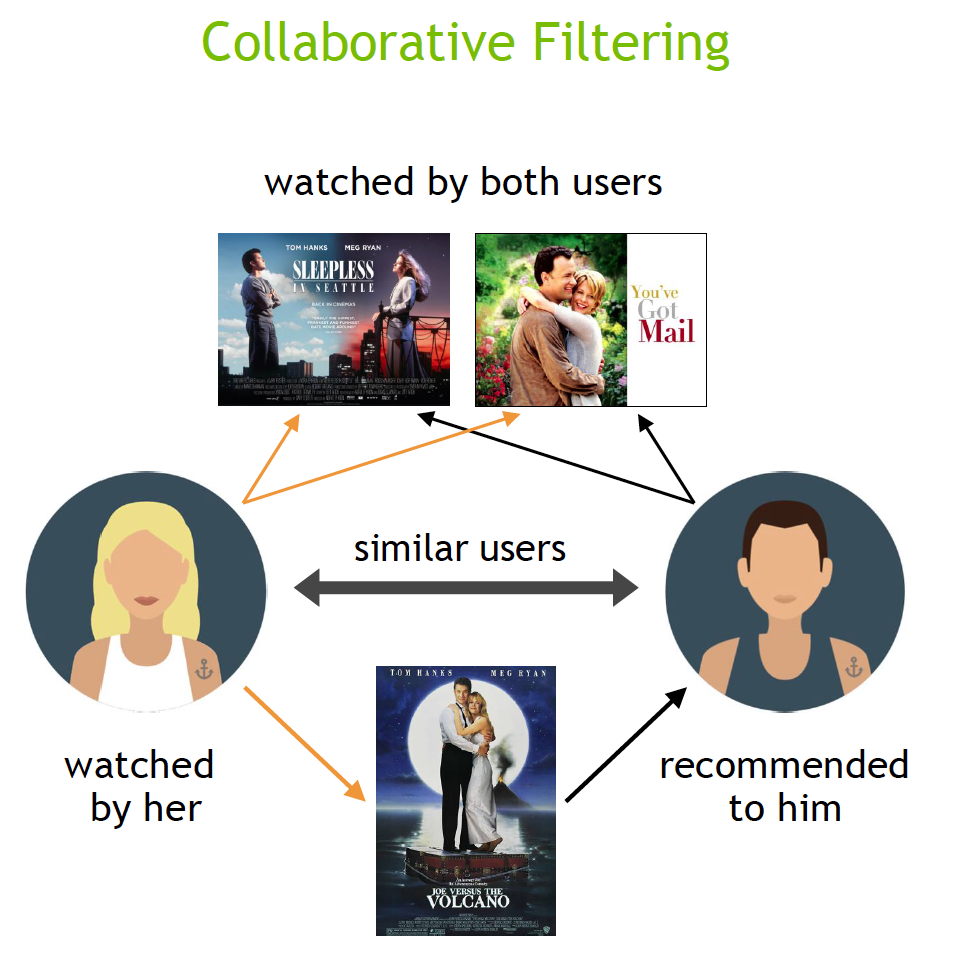
\includegraphics[width=0.4\textwidth]{assets/collaborative_filtering.png}
    \caption{Collaborative Filtering}
    \label{fig:collaborative-filtering}
    \cite{NvidiaRecSys}
\end{figure}

\subsection{Content filtering}\label{subsec:content-filtering}
Content filtering is a technique that uses the features of items a user has interacted with in order to recommend additional items with similar properties. This technique is based on the idea that if a user liked a particular item, he or she will also like an item that is similar to it. 
\begin{figure}[H]
    \centering
    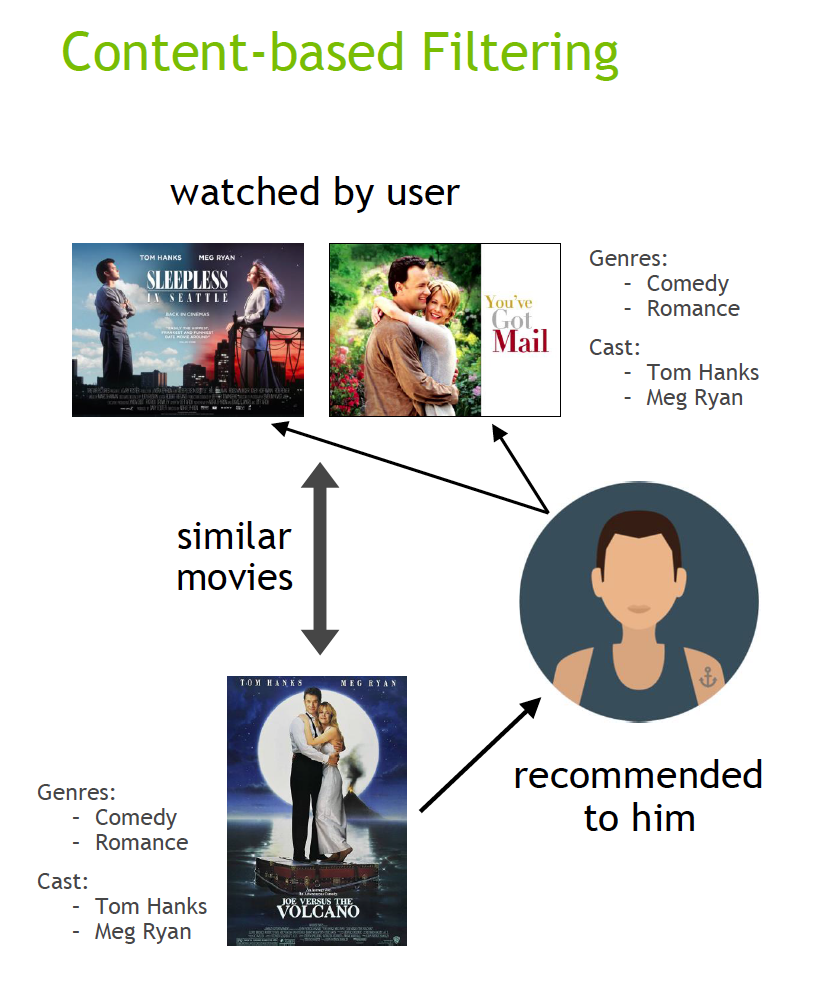
\includegraphics[width=0.4\textwidth]{assets/content_based_filtering.png}
    \caption{Content Filtering}
    \label{fig:content-filtering}
    \cite{NvidiaRecSys}
\end{figure}

\subsection{Hybrid recommendation systems}\label{subsec:hybrid-recommendation-systems}
combine the advantages of the types above to create a more comprehensive recommending system.

\subsection{Context filtering}\label{sec:context-filtering}
Context filtering is a technique that uses the contextual information of the user by framing the recommendation problem as a contextual multi-armed bandit problem and using the contextual information to learn the user's preferences.
\begin{figure}
    \centering
    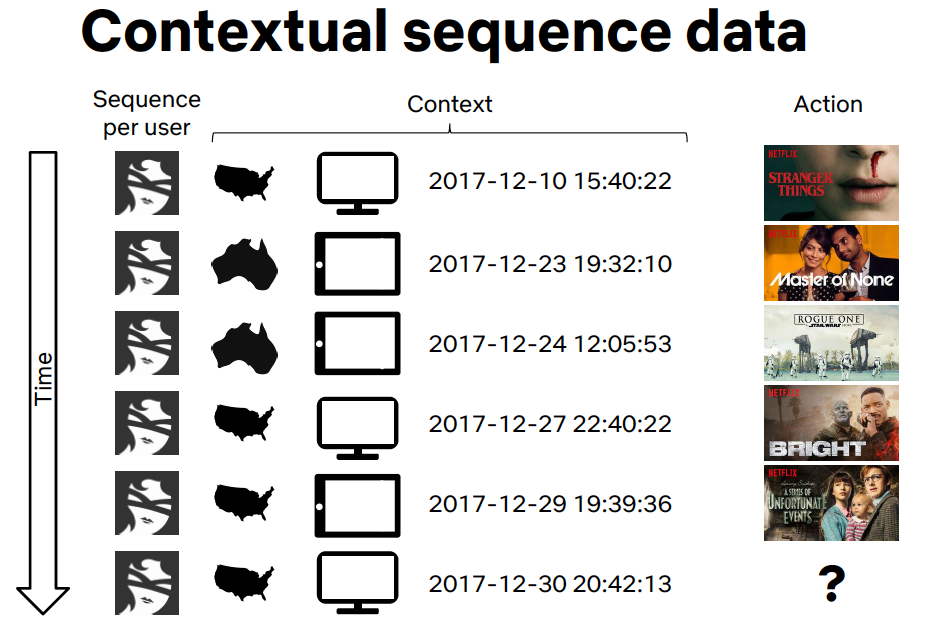
\includegraphics[width=0.5\textwidth]{assets/contextual-sequence-prediction.png}
    \caption{Context Filtering}
    \label{fig:costextual-filtering}
    \cite{NvidiaRecSys}
\end{figure}

\chapter{Literature Review\textemdash ViT Acceleration Techniques}
\minitoc

\section{Pruning}

\section{Quantization}

\section{Low-Rank Approximation}

\section{Knowledge Distillation}

\section{Lightweight ViT}

\section{Transformer Acceleration on Hardware}


\chapter{Proposed Work}
\minitoc


\chapter{Project Plan}
\minitoc


\chapter{Conclusion and Future Work}
\minitoc

\section{Conclusion}

\section{Future Work}

\subsection{Caching Layer}

\cleardoublepage \phantomsection \addcontentsline{toc}{chapter}{Bibliography} \mtcaddchapter
\bibliographystyle{ieeetr.bst}
\bibliography{cites}

\end{document}